\chapter{Background}
\label{Background}
\section{RoboCup}
The RoboCup competition was initially inspired by Hiroaki Kitano~\cite{robocup} in 1993 and his idea eventually led to the establishment of the RoboCup Federation. The RoboCup competition has a bold vision: ``By the year 2050, to develop a team of fully autonomous humanoid robots that can win against the human world soccer champions''. All the teams participating in RoboCup have to find real-time solutions to some of the most difficult problems in robotics (perception, cognition, action, coordination). All the divisions in RoboCup (soccer, RoboCup@Home, RoboRescue, etc.) are designed so as to test the proposed solutions by the various teams to the problems mentioned above. So far, the researchers participating in RoboCup have made a lot of progress in solving real-world problems that show up in the various RoboCup leagues within each division.

\subsection{Standard Platform League}
The Standard Platform League (SPL) is one of the many leagues in the soccer division of RoboCup. In this league all the teams use the same robot, the Aldebaran NAO humanoid robot, and they focus only on algorithm design and software development for this robot. For this reason, the teams are prohibited to make any changes to the hardware of the robot. The robots are completely autonomous and no human intervention from team members is allowed during the games. The only interaction of the robots with the ``outer world'' is the reception of data from the Game Controller, a computer that broadcasts information about the state of the game (score, time, penalties, etc.).

\begin{figure}[t!]
	\begin{center}
		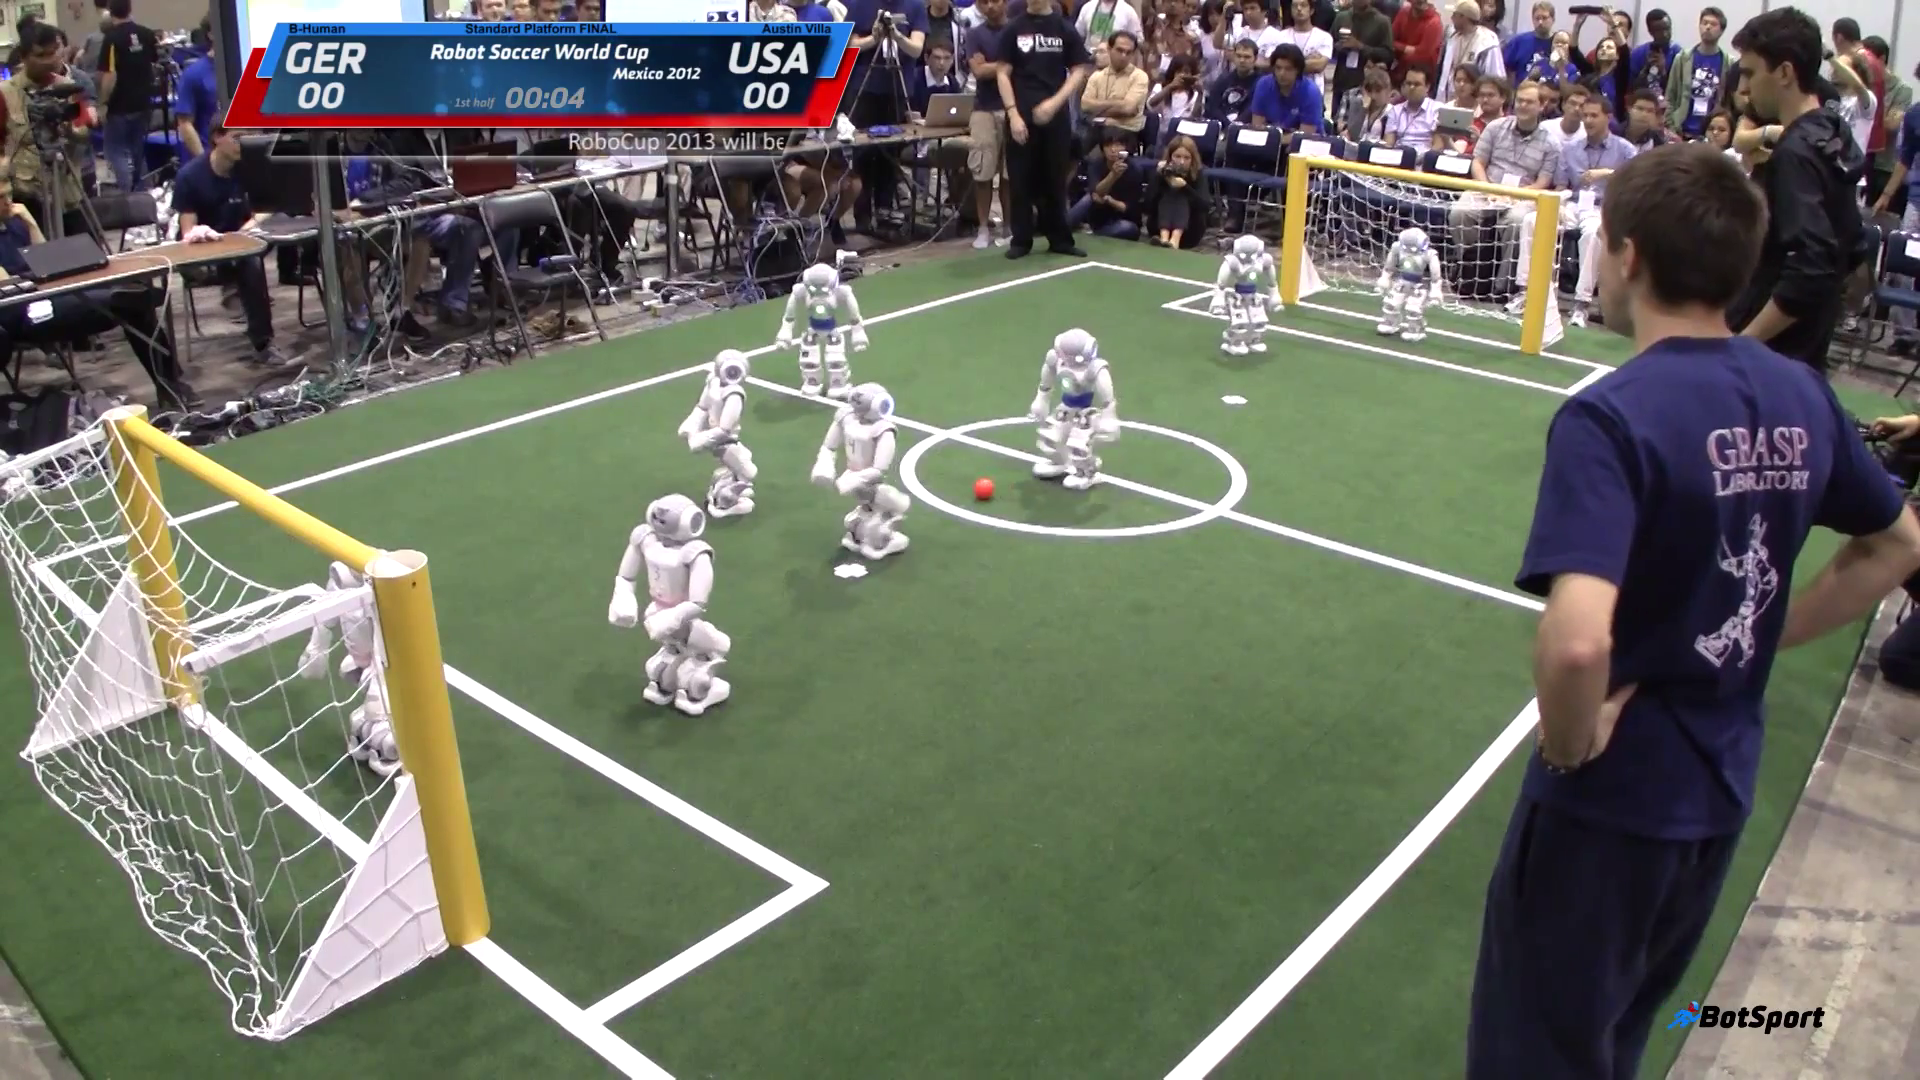
\includegraphics[width=.9\textwidth]{Figures/spl2012.png}
 		\caption{Standard Platform League at RoboCup 2012 (from \url{www.botsport.tv})}
 		\label{fig:RoboCup SPL}
	\end{center}
\end{figure}

Currently, the SPL games are conducted on a field with dimensions \(4m \times 6m\)~\cite{SPLrules2012}. The field consists of a green carpet marked with white lines and two yellow goals (Figure~\ref{fig:RoboCup SPL}). The appearance of the field is similar to a real soccer field, but it is scaled to the size of the robots. The ball is an orange street hockey ball. Each team consists of four robots and each robot carries a colored waist band (blue or pink) that distinguishes the teams. The total game time is 20 minutes and is broken in two halves; each half lasts 10 minutes.




\begin{figure}[t!]
	\begin{center}
		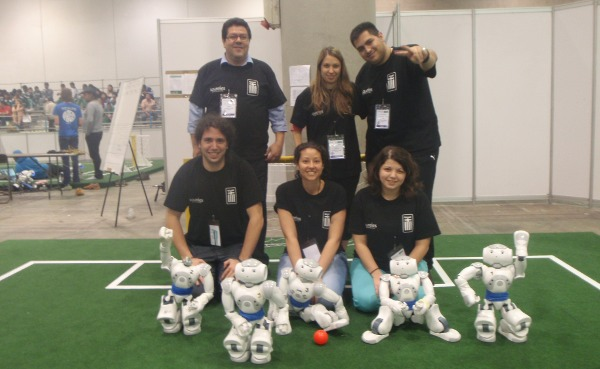
\includegraphics[width=.9\textwidth]{Figures/robocup2012-team.jpg}
 		\caption{Team Kouretes at RoboCup 2012 in Mexico City}
 		\label{fig:Kouretes2012}
	\end{center}
\end{figure}

\section{Robocup SPL Team Kouretes}

Team Kouretes (\url{www.kouretes.gr}) is the RoboCup team of the Technical University of Crete. The team was founded in 2006 and participates in the main RoboCup competition ever since in various leagues (Four-Legged, Standard Platform, MSRS, Webots), as well as in various local RoboCup events (German Open, Mediterranean Open, Iran Open, RC4EW, RomeCup) and RoboCup exhibitions (Athens Digital Week, Micropolis, Schoolfest). In May 2010, the team hosted the 1st official SPL tournament in Greece (with three invited teams) within the Hellenic Conference on Artificial Intelligence (SETN). Distinctions of the team include: {\bf 2nd} place in MSRS at RoboCup 2007; {\bf 3rd} place in SPL-Nao, {\bf 1st} place in SPL-MSRS, among the {\bf top 8} teams in SPL-Webots at RoboCup 2008; {\bf 1st} place in RomeCup 2009; {\bf 6th} place in SPL-Webots at RoboCup 2009; {\bf 2nd} place in SPL at RC4EW 2010; and {\bf 2nd} place in SPL Open Challenge Competition at RoboCup 2011 (joint team Noxious-Kouretes).

The team has been developing its own (publicly-available) software for the Nao robots since 2008. The team code repository includes a custom software architecture, a custom communication framework, graphical tools for monitoring and behavior specification, and modules for object recognition, state estimation, localization, obstacle avoidance, behavior execution, team coordination. The members of the team are senior undergraduate ECE students working on their diploma thesis on a RoboCup-related topic; 15 diploma theses have been completed so far. Recently, the team participated in the RoboCup German Open 2012 competition in Magdeburg, in RoboCup Iran Open 2012 in Tehran, and in RoboCup 2012 in Mexico City (Figure~\ref{fig:Kouretes2012}). In the most recent RoboCup 2012 competition, the team succeeded to proceed to the second round-robin round and rank among the top-16 SPL teams in the world.

\section{Aldebaran NAO Humanoid Robot}
NAO is an integrated, programmable, medium-sized humanoid robot developed by Aldebaran Robotics in Paris, France~\cite{naopaper}. Project NAO started in 2004. In August 2007 NAO officially replaced Sony's AIBO quadruped robot in the RoboCup SPL. In the past few years NAO has evolved over several designs and several versions. 

\begin{figure}[t!]
	\begin{center}
		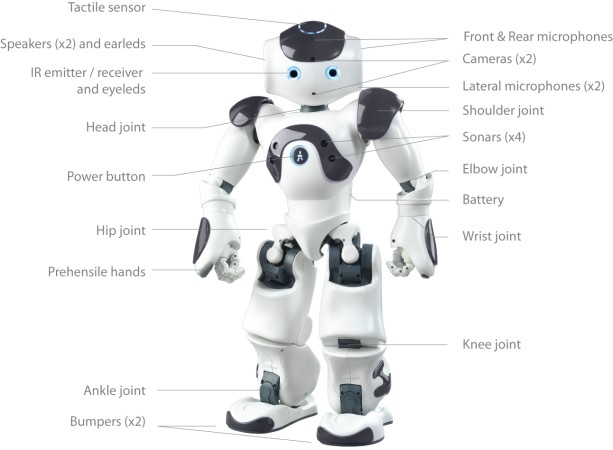
\includegraphics[height = 8cm]{Figures/nao.jpg}
 		\caption{Components of NAO v3.3}
 		\label{fig:sensors}
	\end{center}
\end{figure}

NAO (version V3.3) is a 58cm, 5kg humanoid robot (Figure~\ref{fig:sensors}). The NAO robot carries a fully capable computer on-board with an x86 AMD Geode processor at 500 MHz, 256 MB SDRAM, and 2 GB flash memory running an Embedded Linux distribution. It is powered by a 6-cell Lithium-Ion battery which provides about 30 minutes of continuous operation and communicates with remote computers via an IEEE 802.11g wireless or a wired ethernet link. 

NAO RoboCup edition has 21 degrees of freedom; 2 in the head, 4 in each arm, 5 in each leg and 1 in the pelvis (there are two pelvis joints which are coupled together on one servo and cannot move independently). NAO, also, features a variety of sensors. Two cameras are mounted on the head in vertical alignment providing non-overlapping views of the lower and distant frontal areas, but only one is active each time and the view can be switched from one to the other almost instantaneously. Each camera is a $640 \times 480$ VGA devise operating at 30fps. Four sonars (two emitters and two receivers) on the chest allow NAO to sense obstacles in front of it. In addition, the NAO has a rich inertial unit, with one 2-axis gyroscope and one 3-axis accelerometer, in the torso that provides real-time information about its instantaneous body movements. Two bumpers located at the tip of each foot are simple ON/OFF switches and can provide information on collisions of the feet with obstacles. Finally, an array of force sensitive resistors on each foot delivers feedback of the forces applied to the feet, while encoders on all servos record the actual positions of all joints at each time.



\section{Robot Kinematics}
A \textit{robot kinematic chain} is an articulated manipulator that interacts with the environment and is typically described as an assembly of robotic links connected by (rotary) joints. The joints rotate and control the relative angular positioning of the links of the manipulator. Not all combinations of joints' positions in the chain are valid, because some combinations lead to collisions between the links of the chain or with some fixed item of the environment, such as the floor or a wall. All the valid combinations of joint positions form the \textit{joint space}. The term \textit{degrees of freedom} (DOF) refers to the number of joints in a kinematic chain; clearly, more DOFs imply more flexibility in the motion of the chain. \textit{Robot kinematics} is the application of geometry to the study of  kinematic chains with multiple degrees of freedom. More specifically, robot kinematics provide the transformation from the joint space, where the kinematic chains are defined, to the Cartesian space, where the robot manipulator moves, and vice versa. Robot kinematics are quite useful, because they can be used for planning and executing movements, as well as calculating actuator forces and torques.



\subsection{Forward Kinematics}
The joint space reveals very little information about the position of the end effector of the kinematic chain. The \textit{forward kinematics} define a mapping from the joint space to the three-dimensional Cartesian space. Given a kinematic chain and a set of joint values, forward kinematics can find the point \((p_x,p_y,p_z)\) and the orientation \((a_x,a_y,a_z)\) of the end effector of the kinematic chain in the three-dimensional $x-y-z$ space. Forward kinematics is a domain-independent problem and can be solved for any simple or complex kinematic chain.

\subsection{Inverse Kinematics}
Robot manipulators typically need to reach target points or follow trajectories in the three-dimensional space. To make the end effector reach a point or follow a trajectory, one has to specify appropriate values for the joints of the kinematic chain. Therefore, it is imperative to find ways to go from the three-dimensional space back to the joint space. The \textit{inverse kinematics} define a relation between positions in the three-dimensional space (point \((p_x,p_y,p_z)\) and orientation \((a_x,a_y,a_z)\)) and joint values/angles in the joint space. The problem of inverse kinematics is domain-dependent and every kinematic chain has a different solution. The solution to the inverse kinematics problem can lead to an analytical, closed-form equation or to a numerical, iterative approximation (e.g. with the Jacobian approximation method). As the DOFs increase, each point in the three-dimensional space may have more than one matching point in the joint space. This multiplicity of solutions makes the inverse kinematics a relation, but not a mapping.




\section{Affine Transformations}
An affine transformation is a map transferring points and vectors from one space to another, being able to preserve ratios of distances. The space can be \(n\)-dimensional with \(n\ge2\). The following are affine transformations: Geometric contraction, expansion, dilation, reflection, rotation, shear, similarity transformations, spiral similarities and translation. All the possible combinations of the above produce an affine transformation. Its flexibility concerning object manipulation, makes it a very useful tool in computer graphics.

For the purpose of this thesis we only used rotation and translation, so we will analyze these two types of affine transformation. Also we are working in a three-dimensional space and all the examples from now on will be in this space.

\subsubsection*{Transformation Matrix}
The affine transformation matrix is a \(\left(\left(n+1\right)\times \left(n+1\right)\right)\) matrix where \(n\) is the number of dimensions. In the general form the affine transformation matrix consists of 2 parts:

\[
T = 
\begin{bmatrix}
X & Y \\
\begin{bmatrix}
0 & \cdots & 0
\end{bmatrix} & 1
\end{bmatrix}
\]

X is a (\(n\times n\)) matrix and Y is a (\(n\times 1\)) vector and the last line has \(n-1\) zeros followed by a \(1\). The matrix is invertible if and only if X is invertible and the representation of the inverse is:

\[
T = 
\begin{bmatrix}
X^{-1} & -X^{-1}Y \\
\begin{bmatrix}
0 & \cdots & 0
\end{bmatrix} & 1
\end{bmatrix}
\]

Now if we want to apply the transformation, to a given column vector \(v\), we multiply the affine transformation matrix with the given vector:

\[
v' = Tv = 
\begin{bmatrix}
X & Y \\
\begin{bmatrix}
0 & 0 & 0
\end{bmatrix} & 1
\end{bmatrix}
\begin{bmatrix}
p_x\\
p_y\\
p_z\\
1
\end{bmatrix}
\]

A matrix that is the result of \(n\) multiplications between affine transformation matrices is still an affine transformation. So in the following example, given that all the matrices in the right part of the equation are affine transformation matrices then the resulting matrix T will be an affine transformation matrix.

\[
T = T_1T_2T_3 \cdots T_n
\]

\subsubsection*{Translation Matrix}
Translation, in the Cartesian space, is a function that moves every point by constant distance in a specified direction. We can describe the translation in the three-dimensional space with a (\(4\times4\)) table that has the following form:

\[
A = 
\begin{bmatrix}
1 & 0 & 0 & d_x\\
0 & 1 & 0 & d_y\\
0 & 0 & 1 & d_z\\
0 & 0 & 0 & 1
\end{bmatrix}
\]

The \(d_x,d_y,d_z\) defines the distance that we will move all of our points through the \(x,y,z\) dimension. Obviously, this is an affine transformation matrix with \(X = I\). So now if we want to apply the translation on a given column vector \(v\), we apply it in same way as the transformation:

\[
v' = Tv =
\begin{bmatrix}
1 & 0 & 0 & d_x\\
0 & 1 & 0 & d_y\\
0 & 0 & 1 & d_z\\
0 & 0 & 0 & 1
\end{bmatrix}
\begin{bmatrix}
p_x\\
p_y\\
p_z\\
1
\end{bmatrix}
\]

\subsubsection*{Rotation Matrix}
Rotation matrix is a matrix that is used to perform rotation in Cartesian space. The rotation matrices are always orthogonal matrices with determinant 1.

\[R^T = R^{-1},det(R) = 1\]

In the three-dimensional Cartesian space there are three rotation matrices, each one of them makes a rotation over the \(x\)  or \(y\)  or \(z\) axis. The size of the rotation matrices, for this space, is (\(3\times3\)) and they have the following form:

\[
R_z = 
\begin{bmatrix}
\cos\theta_z & -\sin\theta_z & 0 \\
\sin\theta_z & \cos\theta_z & 0 \\
0 & 0 & 1 
\end{bmatrix}
\]
\[
R_y = 
\begin{bmatrix}
\cos\theta_y & 0 & \sin\theta_y \\
0 & 1 & 0\\
-\sin\theta_y & 0 & \cos\theta_y
\end{bmatrix}
\]
\[
R_x = 
\begin{bmatrix}
1 & 0 & 0 \\
0 & \cos\theta_x & -\sin\theta_x \\
0 & \sin\theta_x & \cos\theta_x
\end{bmatrix}
\]

Now if we want to rotate an object point, defined by the (\(3\times1\)) column vector \(v\), by the \(x\) axis and then by the \(y\) axis we will do the following:

\[
v' = R_xR_yv = 
\begin{bmatrix}
1 & 0 & 0 \\
0 & \cos\theta_x & -\sin\theta_x \\
0 & \sin\theta_x & \cos\theta_x
\end{bmatrix}
\begin{bmatrix}
\cos\theta_y & 0 & \sin\theta_y \\
0 & 1 & 0\\
-\sin\theta_y & 0 & \cos\theta_y
\end{bmatrix}
\begin{bmatrix}
p_x\\
p_y\\
p_z
\end{bmatrix}
\]

We can use combinations of those 3 matrices and make other useful rotation matrices. For example we can construct the rotation matrix that rotates all the axes with the following order, first the \(z\) axis then the \(y\) axis and finally the \(x\) axis.

\[
	R = R_zR_yR_x
\]

The analytical form of the above rotation matrix:

\[
R = 
\begin{bmatrix}
\cos\theta_y\cos\theta_z & -\cos\theta_x\sin\theta_z + \sin\theta_x\sin\theta_y\cos\theta_z & \sin\theta_x\sin\theta_z + \cos\theta_x\sin\theta_y\cos\theta_z\\

\cos\theta_y\sin\theta_z & \cos\theta_x\cos\theta_z + \sin\theta_x\sin\theta_y\sin\theta_z & -\sin\theta_x\cos\theta_z + \cos\theta_x\sin\theta_y\sin\theta_z\\

-\sin\theta_y & \sin\theta_x\cos\theta_y & \cos\theta_x\cos\theta_y
\end{bmatrix}
\]

Finally we can easily transform a rotation matrix to an affine transformation matrix just by padding with zeros and an one in the corner. So from now on whenever we use a rotation matrix, this matrix will have the following form:

\[
R' = 
\begin{bmatrix}
R &  \begin{bmatrix} 0\\0\\0 \end{bmatrix}\\
\begin{bmatrix}
0 & 0 & 0
\end{bmatrix} & 1
\end{bmatrix}
\]


\subsubsection*{Affine Transformation Matrix in this Thesis}
In this thesis we are using the rotation and the translation matrix so we can move points in the three-dimensional space. We can assume that our affine transformation matrix is composed by a rotation and a translation matrix. The affine transformation matrix, that we will work with, has \(X = R\) and \(Y = v\) where \(v\) is the vector with the distance points from the translation matrix.

\[
T = 
\begin{bmatrix}
R &  \begin{bmatrix} p_x\\p_y\\p_z \end{bmatrix}\\
\begin{bmatrix}
0 & 0 & 0
\end{bmatrix} & 1
\end{bmatrix}
\] 

Also we can decompose this transformation matrix to a rotation matrix followed by a translation matrix. Given a rotation \(R\) and a translation matrix \(A\):

\[R = 
\begin{bmatrix}
R &  \begin{bmatrix} 0\\0\\0 \end{bmatrix}\\
\begin{bmatrix}
0 & 0 & 0
\end{bmatrix} & 1
\end{bmatrix}
\]
\[A = 
\begin{bmatrix}
I &  \begin{bmatrix} p_x\\p_y\\p_z \end{bmatrix}\\
\begin{bmatrix}
0 & 0 & 0
\end{bmatrix} & 1
\end{bmatrix}
\]

The result from the multiplication of \(R\) with \(A\) is:

\[
T = RA = 
\begin{bmatrix}
R &  R\begin{bmatrix} p_x\\p_y\\p_z \end{bmatrix}\\
\begin{bmatrix}
0 & 0 & 0
\end{bmatrix} & 1
\end{bmatrix}
\]

So we can assume that the translation matrix \(A'\) is:

\[
A' = 
\begin{bmatrix}
I &  R\begin{bmatrix} p_x\\p_y\\p_z \end{bmatrix}\\
\begin{bmatrix}
0 & 0 & 0
\end{bmatrix} & 1
\end{bmatrix}
\]

Now if we multiply \(A'\) with the \(R\) we will have the same transformation matrix as before:
 
\[
A'R = 
\begin{bmatrix}
I &  R\begin{bmatrix} p_x\\p_y\\p_z \end{bmatrix}\\
\begin{bmatrix}
0 & 0 & 0
\end{bmatrix} & 1
\end{bmatrix}
\begin{bmatrix}
R &  \begin{bmatrix} 0\\0\\0 \end{bmatrix}\\
\begin{bmatrix}
0 & 0 & 0
\end{bmatrix} & 1
\end{bmatrix}
= 
\begin{bmatrix}
R &  R\begin{bmatrix} p_x\\p_y\\p_z \end{bmatrix}\\
\begin{bmatrix}
0 & 0 & 0
\end{bmatrix} & 1
\end{bmatrix} =
RA
\]

\section{DH (Denavit-Hartenberg) Parameters}
Denavit and Hartenberg found a way to create a transformation matrix that describes points in one end of the joint to a coordinate system that is fixed to the other end, as a function of the joint state~\cite{dhparam1,dhparam2,introroboticscraigbook}. They found that we can construct this transformation matrix using only 4 parameters, the DH (Denavit-Hartenberg) Parameters. These parameters are: 

\[a,\alpha,d \text{ and } \theta\]

Before we can explain these parameters we must first establish the reference frame of each joint respectively to the previous joint reference frame.

\begin{itemize}
\item The \(z_n\)-axis is in the direction of the joint axis. 
\item The \(x_n\)-axis is parallel to the common normal: \(x_n = z_n \times z_{n-1}\). The direction of \(x_n\) is from \(z_{n - 1}\) to \(z_n\).
\item The \(y_n\)-axis follows from the \(x_n\)  and \(z_n\)-axis by choosing it to be a right-handed coordinate system.
\end{itemize}

Now we can describe the DH parameters as following:

\begin{itemize}
\item\(a\): length of the common normal.
\item\(alpha\): angle about common normal, from \(z_{n-1}\)-axis to \(z_n\)-axis.
\item\(d\): offset along \(z_{n-1}\) to the common normal.
\item\(\theta\): angle about \(z_{n-1}\), from \(x_{n-1}\) to \(x_n\).
\end{itemize}

There is a great site with that explains the way to find those parameters and has some videos to visualize the explanation~\cite{tekkotsu}.
Now we can go from one reference frame to the other by composing the transformation matrix:

\[DH = R_x(\alpha)T_x(a)R_z(\theta)T_z(d)\]

The analytical form of the resulting matrix from the above composition is:

\[
DH = 
\begin{bmatrix}
\cos\theta & -\sin\theta & 0 & a\\
\sin\theta\cos\alpha & \cos\theta\cos\alpha & -\sin\alpha & -d\sin\alpha\\
\sin\theta\cos\alpha & \cos\theta\sin\alpha & \cos\alpha & d\cos\alpha\\
0 & 0 & 0 & 1
\end{bmatrix}
\]

We can notice that the above transformation matrix is an affine transformation matrix because it is the product of the multiplication of affine transformation matrices.

\section{Mathematica}
Mathematica$^{\textrm{\copyright}}$ is a software tool for mathematic computations created by the Wolfram company (\url{http://www.wolfram.com/}). It is very useful, because it can find solution to differential equations and can very easily execute symbolic computations. For the purpose of this thesis, we want a software with the capability to perform fast and large symbolic computations with matrices. Also it has the capability to simplify the symbolic results really fast.

The following code is a small example for the symbolic computation. We construct two matrices with cosines and sines and we have two symbols, theta1 and theta2. Next we just do the multiplication between those to matrices and we simplify the result:

\begin{scriptsize}
\begin{verbatim}
Matrix1 = {{Cos[theta1], -Sin[theta1]}, {Cos[theta1], -Cos[theta1]}};
Matrix2 = {{Cos[theta2], -Sin[theta2]}, {Cos[theta2], -Cos[theta2]}};
T = Matrix1.Matrix2;
Simplify[T];
MatrixForm[%]
\end{verbatim}
\end{scriptsize}
The symbolic computations are the following:
\begin{small}
\begin{align*}
\text{Matrix1} &= \begin{bmatrix}
\cos\theta_1 & -\sin\theta_1\\
\cos\theta_1 & -\cos\theta_1
\end{bmatrix}\\
\text{Matrix2} &= \begin{bmatrix}
\cos\theta_2 & -\sin\theta_2\\
\cos\theta_2 & -\cos\theta_2
\end{bmatrix}\\
\text{T} &= \begin{bmatrix}
\cos\theta_1\cos\theta_2 - \cos\theta_2\sin\theta_1 &   \cos\theta_2 \sin\theta_1 - \cos\theta_1 \sin\theta_2\\
0 & \cos\theta_1 \cos\theta_2 - \cos\theta_1 \sin\theta_2
\end{bmatrix}\\
\text{T}_{\text{simplified}} &= \begin{bmatrix}
\cos\theta_2\left(\cos\theta_1 - \sin\theta_1\right) & \sin\left(\theta_1 - \theta_2\right)\\
 0 & \cos\theta_1 \left(\cos\theta_2 - \sin\theta_2\right)
\end{bmatrix}
\end{align*}\\
\end{small}

The example above is very simple, but illustrates the Mathematica simplification step, which is very importand for our work, where he have to deal with much larger and more complex matrices.